\documentclass[a4paper,10pt,ngerman]{scrartcl}
\usepackage{babel}
\usepackage[T1]{fontenc}
\usepackage[utf8x]{inputenc}
\usepackage[a4paper,margin=2.5cm,footskip=0.5cm]{geometry}

% Die nächsten drei Felder bitte anpassen:
\newcommand{\Aufgabe}{Aufgabe 2: Simultane Labyrinthe} % Aufgabennummer und Aufgabennamen angeben
\newcommand{\TeilnahmeId}{74749}                  % Teilnahme-ID angeben
\newcommand{\Name}{Christian Krause}             % Name des Bearbeiter / der Bearbeiterin dieser Aufgabe angeben

\usepackage{siunitx}
% Kopf- und Fußzeilen
\usepackage{scrlayer-scrpage, lastpage}
\setkomafont{pageheadfoot}{\large\textrm}
\lohead{\Aufgabe}
\rohead{Teilnahme-ID: \TeilnahmeId}
\cfoot*{\thepage{}/\pageref{LastPage}}

% Position des Titels
\usepackage{titling}
\setlength{\droptitle}{-1.0cm}

% Für mathematische Befehle und Symbole
\usepackage{amsmath}
\usepackage{amssymb}

% Für Bilder
\usepackage{graphicx}

% Für Algorithmen
\usepackage{algorithm}      % floating wrapper for algorithms
\usepackage{algpseudocode}
\usepackage{hyperref}

% Für Quelltext
\usepackage{listings,listings-rust}

\usepackage{fontspec}
\setmonofont{JetBrains Mono}[
    Contextuals = Alternate,
    Ligatures = TeX,
]
\usepackage[%
    backend=biber,
    style=authortitle,
    sorting=nyt,
]{biblatex}
\addbibresource{main.bib}
\lstset{
    basicstyle = \ttfamily,
    columns = flexible,
}
\makeatletter
\renewcommand*\verbatim@nolig@list{}
\makeatother


\definecolor{mygreen}{rgb}{0,0.6,0}
\definecolor{mygray}{rgb}{0.5,0.5,0.5}
\definecolor{mymauve}{rgb}{0.58,0,0.82}
\lstset{
    keywordstyle=\color{blue},commentstyle=\color{mygreen},
    stringstyle=\color{mymauve},rulecolor=\color{black},
    basicstyle=\footnotesize\ttfamily,numberstyle=\tiny\color{mygray},
    captionpos=b, % sets the caption-position to bottom
    keepspaces=true, % keeps spaces in text
    numbers=left, numbersep=5pt, showspaces=false,showstringspaces=true,
    showtabs=false, stepnumber=2, tabsize=2, title=\lstname
}
\lstdefinelanguage{JavaScript}{ % JavaScript ist als einzige Sprache noch nicht vordefiniert
    keywords={break, case, catch, continue, debugger, default, delete, do, else, finally, for, function, if, in, instanceof, new, return, switch, this, throw, try, typeof, var, void, while, with},
    morecomment=[l]{//},
    morecomment=[s]{/*}{*/},
    morestring=[b]',
    morestring=[b]",
    sensitive=true
}
% Diese beiden Pakete müssen zuletzt geladen werden
%\usepackage{hyperref} % Anklickbare Links im Dokument
\usepackage{cleveref}

% Daten für die Titelseite
\title{\textbf{\Huge\Aufgabe}}
\author{\LARGE Teilnahme-ID: \LARGE \TeilnahmeId \\\\
\LARGE Bearbeiter/-in dieser Aufgabe: \\
\LARGE \Name\\\\}
\date{\LARGE\today}

\begin{document}

    \maketitle
    \tableofcontents

    \vspace{0.5cm}


    \section{Lösungsidee}
    Ich habe mich damit beschäftigt, einen Algorithmus zu entwickeln, der eine optimale Lösung für die Aufgabenstellung berechnen kann.
    Eine optimale Lösung ist hier die kürzeste Anweisungssequenz, die Anton und Bea ins Ziel bringt.
    In diesem Abschnitt wird direkt der Aufgabenteil b) behandelt, der Algorithmus ist aber auch für Labyrinthe ohne Gruben geeignet.

    \subsection{Modellierung}
    Im folgenden arbeite ich mit der Annahme, dass die Labyrinthe von Wänden umgeben sind. \\
    Jeder Zustand, in dem sich Anton und Bea befinden, kann als Tupel der jeweiligen Koordinaten dargestellt werden: $((x_0,y_0), (x_1, y_1))$.
    $(x_0,y_0)$ ist hier die Position von Anton (der sich in Labyrinth 1 befindet), $(x_1, y_1)$ beschreibt die Position von Bea im zweiten Labyrinth.
    Am Anfang herrscht der Zustand $S_0 = ((0,0), (0,0))$, da sich beide auf ihrem Startfeld befinden. Chris kann nun vier mögliche Anweisungen geben, die einen neuen Zustand herbeiführen würden. Wenn Anton und Bea beide ihr Zielfeld erreicht haben, befindet wir uns in dem Zustand $S_{end} = ((n-1, m-1), (n-1, m-1))$.\\
    Formal können die verschiedenen Positionen von Anton und Bea als Graph dargestellt werden, dessen Knoten alle Möglichen Zustände sind.
    \[ V = \{((x_0, y_0), (x_1, y_1)) \in ((\mathbb{N} \times \mathbb{N}) \times (\mathbb{N} \times \mathbb{N}))\mid 0 \le x_0, x_1 < n \land 0 \le y_0, y_1 < m\}\]
    Von jedem Knoten gehen vier Kanten aus, eine für jede Anweisung, die Chris geben könnte. Die Menge der Anweisungen $A$ kann formal als Menge an Funktionen dargestellt werden, die eine Position $p = (x_0, y_0)$ in eine neue Position $p'$ (die oben, unten, rechts oder links von $p$ ist) überführt: \[A = \{(x_0, y_0) \mapsto (x_0 + 1, y_0), (x_0, y_0) \mapsto (x_0 - 1, y_0), (x_0, y_0) \mapsto (x_0, y_0 + 1), (x_0, y_0) \mapsto (x_0, y_0 - 1)\}\]
    Ob Anton und Bea diese Anweisung ausführen können, hängt natürlich davon ab, ob sie die neue Position erreichen können, ohne gegen eine Wand zu stoßen oder in eine Grube zu fallen. Formal führen Anton und Bea an der Position $p$ bei jeder Anweisung $a \in A$ folgende Funktion aus, um ihre neue Position $p'$ zu bestimmen:
    \[p' = f(p, a) =
    \begin{cases}
        p & \parbox[t]{.6\textwidth}{Falls zwischen $p$ und $a(p)$ eine Wand ist oder \\ das Zielfeld erreicht ist (also $p = (n-1, m-1)$).} \\
        (0, 0)  & \text {Falls $a(p)$ eine Grube ist.}\\
        a(p) & \text{ansonsten} \\
    \end{cases}\]
    Da wir annehmen, dass das Labyrinth von Wänden umgeben ist, gibt es keine Position $p$, von der aus man mit einer Anweisung $a \in A$, eine Position $f(p,a)$ erreichen kann, die außerhalb des Labyrinths liegt. \\
    Um auf die zwei Positionen eines Zustands $S \in V, S = (p_0, p_1)$ zuzugreifen, schreibe ich ab jetzt $S[0] = p_0$ für die Position von Anton und $S[1] = p_1$ für die Position von Bea.\\
    Die Zustandsänderung des Zustands $S \in V$, die durch die Anweisung $a \in A$ hervorgerufen wird, ist also: \[S' = (f(S[0], a), f(S[1], a)).\] Zwischen zwei Zuständen $S \in V$ und $S' \in V$ existiert also eine Kante, wenn $S'$ durch die Anwendung einer Anweisung $a \in A$ auf $S$ erreicht werden kann:
    \[E = \{(S, S') \in (V \times V) \mid \exists a \in A, S' = (f(S[0], a), f(S[1], a)\}\]
    Eine Kante zwischen dem Startknoten $S$ und dem Endknoten $S'$ wird hier als Tupel $(S, S')$ dargestellt.\\
    Alle Kanten haben die Länge $1$, da sie genau einer Anweisung entsprechen. \\
    Jeder Pfad von einem Knoten $A \in V$ zu einem anderen Knoten $B \in V$ repräsentiert eine Sequenz von Anweisungen, die Anton und Bea von ihren Positionen bei $A$ zu ihren Positionen bei $B$ bringt.
    Die Länge eines solchen Pfades entspricht der Anzahl der durchlaufenen Anweisungen.\\
    Der kürzeste Pfad von $S_0$ zu $S_{end}$ entspricht also einer kürzesten Anweisungssequenz, die Anton und Bea ins Ziel bringt. Die Aufgabenstellung lässt sich also darauf reduzieren, den kürzesten Pfad von $S_0$ zu $S_{end}$ in dem oben beschriebenen Graph zu finden. \\
    Da der Graph nicht gewichtet ist, kann dieser Pfad mit einer Breitensuche gefunden werden.\\


    \section{Breitensuche}



    In der Implementierung können alle Schleifen, also Kanten die einen Knoten mit sich selbst verbinden, ignoriert werden, da sie mit Anweisungen zusammenhängen, die den Zustand nicht ändern (z.B. da Anton und Bea beide gegen eine Wand laufen). \\
    Außerdem muss man beachten, dass Anton und Bea warten, wenn sie ihr Zielfeld bereits erreicht haben. Wenn also eine der Koordinaten die Position $(n-1,m-1)$ erreicht hat, wird diese von den Anweisungen von Chris nicht mehr verändert. Da nun nur noch eine Person ihr Ziel finden muss, würde es keinen Sinn machen, Anwendungen auszuführen, mit denen diese Person gegen eine Wand laufen würde. Dies muss aber in der Praxis nicht extra überprüft werden, da sich der Gesamtzustand in diesen Fällen nicht ändern würde (da eine Person gegen die Wand läuft und die andere wartet). Solche Anweisungen werden sowieso herausgefiltert.
        \begin{algorithm}[H]
        \begin{algorithmic}[1]
            \Function{BFS}{Labyrinth1, Labyrinth2}
                \State visited $\gets$ leeres Dictionary
                \State visited[$S_0$] $\gets$ null
                \State queue $\gets$ leere Warteschlange
                \State queue.\Call{enqueue}{$S_0$}

                \While{queue nicht leer}
                    \State S $\gets$ queue.\Call{popfirst}{}
                    \If{$S = S_{end}$}
                        \State \textbf{break}
                    \EndIf
                    \For{jede Anweisung $a \in A$}
                        \State S' $\gets$ (f(S[0], a), f(S[1], a))
                        \If{$S' = S$}
                            \State \textbf{continue}
                        \EndIf
                        \If{$S' \in$  visited}
                            \State \textbf{continue}
                        \EndIf
                        \State visited[$S'$] $\gets$ $S$
                        \State queue.\Call{enqueue}{S'}
                    \EndFor
                \EndWhile
                \If{$S_{end} \notin$ visited}
                    \State \Call{Print}{``No path found''}
                \Else
                    \State \Return \Comment{Verfolge Pfad anhand der visited Hashmap zurück}
                \EndIf
            \EndFunction
        \end{algorithmic}\label{alg:bfs}
    \end{algorithm}
    Am Anfang werden die Variablen \textit{visited} und \textit{queue} initialisiert. Die \textit{visited}-Variable ist eine Hashmap, die alle Knoten speichert, die bereits besucht wurden. Der Schlüssel ist der Knoten, der besucht wurde und der Wert ist der Knoten, von dem aus dieser Knoten erreicht wurde. Die \textit{queue} ist eine Warteschlange, die alle Knoten speichert, die noch besucht werden müssen.\\
    In der While-Schleife wird immer der erste Knoten $S$ aus der Warteschlange entfernt.
    Falls dieser der Zielknoten ist, ist die Suche abgeschlossen.\\
    Ansonsten wird für jede Anweisung der Zustand $S'$ berechnet, der durch die Anwendung der Anweisung auf $S$ erreicht werden kann.
    Falls dieser Zustand $S$ nicht ändert (weil Anton und Bea gegen die Wand laufen) oder schon besucht wurde, wird die Anweisung übersprungen.\\
    Ansonsten wird $S'$ in die \textit{visited}-Hashmap eingetragen und zur Warteschlange hinzugefügt.\\
    Wenn die Warteschlange leer ist, aber der Zielknoten nicht besucht wurde, gibt es keinen Pfad von $S_0$ zu $S_{end}$ und die Suche wird abgebrochen.
    Falls ein Pfad gefunden wurde, kann er anhand der \textit{visited} Hashmap zurückverfolgt werden.

    \subsubsection{Laufzeitkomplexität}
    Im Worst-Case besucht die Breitensuche jeden Knoten genau einmal, die While-Schleife wird also $O(\|V\|)$ mal ausgeführt.
    Die For-Schleife in der While-Schleife läuft für jede Anweisung einmal, also $O(4) = O(1)$ mal.
    Da die Operationen in der For-Schleife (mit der Hashmap und der Warteschlange) mit einer theoretischen Laufzeit von $O(1)$ ausgeführt werden können, ist die Laufzeit der For-Schleife insgesamt $O(1)$.
    Damit hat der gesamte Algorithmus eine Laufzeit von $O(\|V\|)$. \\
    Der oben beschriebene Graph besitzt einen Knoten für jede Mögliche Kombination an Positionen von Anton und Bea.
    Bea und Anton können jeweils $n \cdot m$ verschiedene Positionen einnehmen, d.h. insgesamt hat der Graph $\|V\| = n^2 m^2$ Knoten, d.h. die Laufzeit ist $O(n^2 m^2)$. \\
    Das stimmt auch mit der allgemein bekannten Laufzeit für Breitensuche von $O(\|E\| + \|V\|)$ überein, da jeder Knoten höchstens vier ausgehende Kanten hat: $\|E\| \le 4 \cdot n ^2 m^2$.
    Die Wort-Case Laufzeit ist also: \[O(n^2 m^2 + 4 \cdot n^2 m^2) = O(n^2 m^2).\]
    Die Breitensuche hat im Wort-Case einen Speicherplatzverbrauch von $O(\|V\|) =  O(n^2 m^2)$, da alle besuchten Knoten in der \textit{visited}-Hashmap gespeichert werden müssen.

    \subsection{Bidirektionale Breitensuche}
    Die Breitensuche hat die bestmögliche asymptotische Laufzeit für einen Algorithmus, der einen optimalen Pfad in einem Graphen findet, der nicht gewichtet ist. \\
    In der Praxis lässt sie sich aber noch weiter optimieren, nämlich durch das Verfahren der Bidirektionalen Breitensuche.
    Dabei wird die Breitensuche nicht nur von dem Startknoten $S_0$ aus gestartet, sondern gleichzeitig auch \glqq rückwärts\grqq~von $S_{end}$ aus.
    Sobald die Breitensuche aus der einen Richtung einen Knoten besucht, der von der anderen Richtung aus schon besucht wurde, ist ein kürzester Pfad gefunden und die Suche ist abgeschlossen.
    Dabei muss aber genauer auf die Reihenfolge geachtet werden, in der die Knoten besucht werden.
    Die normale Breitensuche funktioniert nämlich mit einer Datenstruktur, die wie eine Warteschlange (Queue) nach dem First-in Last-out prinzip funktioniert. Das bedeutet, dass ein neuer Knoten, der zu der Warteschlange hinzugefügt wurde erst besucht wird, wenn alle anderen Knoten, die vorher hinzugefügt wurden bereits aus der Warteschlange entfert sind.
    Das bedeutet, dass zuerst alle Knoten, die $i$ Kanten von $S_0$ entfernt sind, besucht werden, bevor ein Knoten in der Entfernung $i+1$ besucht wird.
    Daraus folgt auch die Optimalität der Breitensuche, da so sicher der kürzeste Pfad gefunden wird. \\

    Würde man bei der bidirektionalen Breitensuche dieses Verfahren vom Startknoten aus und vom Zielknoten aus rückwärts anwenden, könnte es passieren, dass ein Pfad gefunden wird, der um eine Kante zu lang ist. \\
    Darum müssen die Knoten von jeder Breitensuche aus \glqq Ebene für Ebene\grqq~besucht werden:
    \begin{algorithm}[H]
        \caption{Bidirektionale Suche}
        \label{alg:bidirectional-search}
        \begin{algorithmic}[1]
            \State $Visited_{1} \gets \{S_{0}\}$
            \State $Visited_{2} \gets \{S_{\text{end}}\}$
            \State $Frontier_{1} \gets \{S_{0}\}$
            \State $Frontier_{2} \gets \{S_{\text{end}}\}$
            \While{$|Frontier_{1}| > 0 \,\land\, |Frontier_{2}| > 0$}
                \If{$|Frontier_{1}| \le |Frontier_{2}|$}
                    \State $Frontier_{1} \gets \text{Expand\_by\_one}_1(Frontier_{1})$
                    \State $Visited_{1} \gets Visited_{1} \cup Frontier_{1}$
                    \If{$|Frontier_{1} \,\cap\, Visited_{2}| > 0$}
                        \State \textbf{exit} \Comment{Pfad gefunden!}
                    \EndIf
                \Else
                    \State $Frontier_{2} \gets \text{Expand\_by\_one}_2(Frontier_{2})$
                    \State $Visited_{2} \gets Visited_{2} \cup Frontier_{2}$
                    \If{$|Frontier_{2} \,\cap\, Visited_{1}| > 0$}
                        \State \textbf{exit} \Comment{Pfad gefunden!}
                    \EndIf
                \EndIf
            \EndWhile
        \end{algorithmic}
    \end{algorithm}
    Als erstes werden die Variablen \textit{Visited$_1$} und \textit{Visited$_2$} initialisiert, um die Knoten zu speichern, für die bereits ein Pfad von $S_0$ bzw von $S_{end}$ aus bekannt ist. Die Variablen \textit{Frontier$_1$} und \textit{Frontier$_2$} speichern alle Knoten, die genau $i$ Pfadlängen von $S_0$ bzw $S_{end}$ entfernt sind. In der Schleife wird entschieden, ob die Binärsuche von $S_0$ aus oder die von $S_{end}$ aus um eine Ebene weitergeführt werden. In welcher Reihenfolge dies geschieht ist irrelevant, der Algorithmus ist in jedem Fall optimal. Hier wird die Seite weitergeführt, die zurzeit weniger \glqq aktive\grqq~Knoten hat, die erweitert werden sollen.\\
    Die $\textit{Expand\_by\_one}_1$ Funktion nimmt eine Menge an Knoten und gibt alle Knoten zurück, die genau eine Pfadlänge von einem der Knoten in \textit{Frontier} entfernt liegen, was einem Schritt der Binärsuche entspricht. Die Funktion $\textit{Expand\_by\_one}_1$ geht dabei entlang der Pfeile des Graphen und $\textit{Expand\_by\_one}_2$ geht \glqq Rückwärts\grqq~in die entgegengesetzte Richtung. \\
    Anschließend werden in beiden Fällen die neuen Knoten zur jeweiligen \textit{Visited}-Menge hinzugefügt.
    Am Ende wird überprüft, ob einer der neuen Knoten in der jeweiligen \textit{Frontier}-Variable bereits aus der anderen Richtung besucht wurde. Wenn dies der Fall ist, dann ist der kürzeste Pfad gefunden, da zu dem Knoten, der nun z.B. in $\textit{Frontier}_1$ und $\textit{Visited}_2$ enthalten ist, ein Pfad von $S_0$ aus und von $S_{end}$ aus bekannt ist. Im Umsetzungsteil gehe ich genauer darauf ein, welche Möglichkeiten es gibt, diesen Pfad zu speichern und zurückzuverfolgen.

    \subsubsection{Optimalität}
    Warum??

    \subsubsection{Laufzeit}
    Asymptotisch ist die Laufzeit von bidirektionaler Breitensuche gleich wie die der normalen Breitensuche, im Wort-Case muss jeder Knoten und jede Kante besucht werden, also $O(\|V\| + \|E\|)$.
    \begin{figure}[H]
        \label{fig:1}
        \centering
        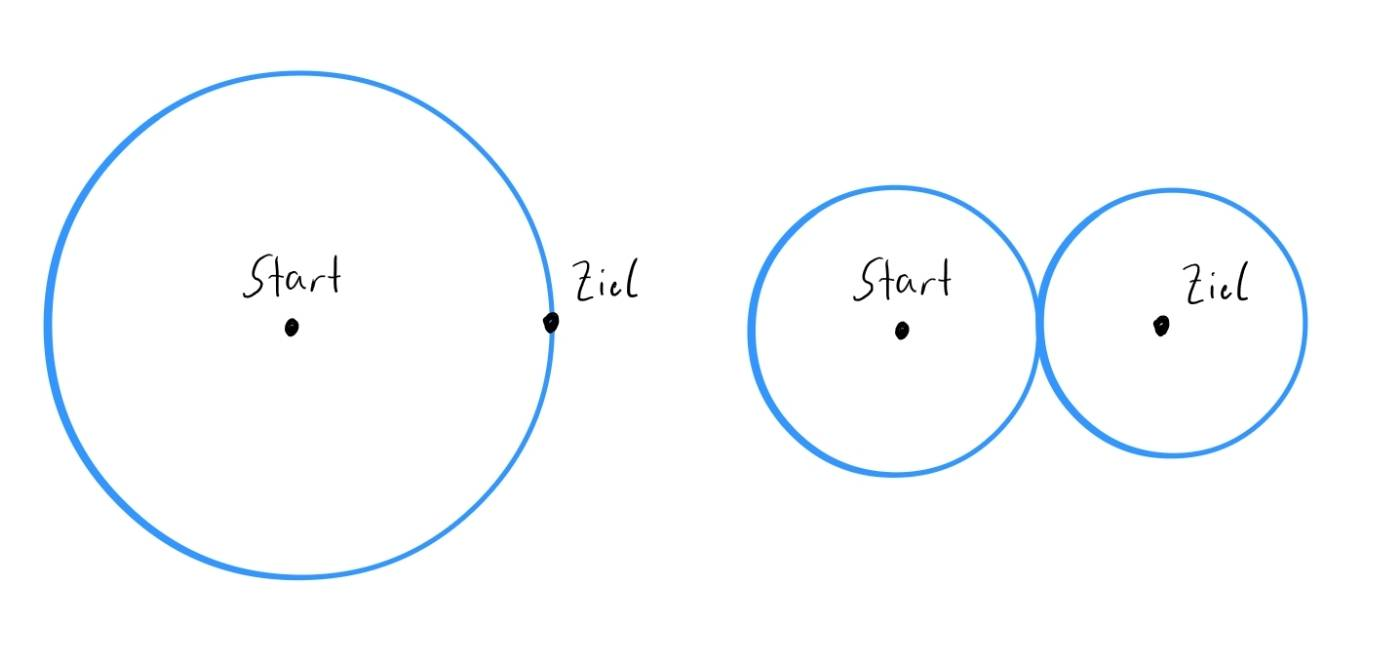
\includegraphics[width=0.7\textwidth]{Assets/zeichnung}
        \caption {Links: normale Breitensuche, Rechts: Bidirektionale Breitensuche}
    \end{figure}

    Intuitiv ist Bidirektionale Breitensuche aber schneller, da meistens weniger Knoten besucht werden müssen (siehe Bild \ref{fig:1}). \\
    Mathematisch lässt sich das schwer quantifizieren, man kann allerdings eine andere Obergrenze der Laufzeit der Breitensuche betrachten. Sei $d$ die Länge des Pfades, der gefunden werden muss und $b$ die Durchschnittliche Anzahl an ausgehenden Kanten eines Knotens, in unserem Fall $d = 4$.
    Die Laufzeit von Breitensuche lässt sich durch $O(b^d)$ begrenzen, da, bis der Zielknoten gefunden wurde, auf jeder \glqq Ebene\grqq die Anzahl der besuchten Knoten um den Faktor $b$ steigt.\\
    Die zwei Breitensuchen der Bidirektionalen Breitensuche treffen sich aber schon nach $D/2$ Schritten in der Mitte (wenn man beide Richtungen immer abwechselnd um eine Ebene erweitert).
    Die Laufzeit der Bidirektionalen Breitensuche lässt sich also durch $O(b^{\frac d 2})$ begrenzen. \\
    Für die Pfadlänge in unserem Graphen gilt allerdings $d > m + n$, und da $m^2 n^2  \le 4^{\frac {n + m} 2}$ für alle $n, m \in \mathbb N$ ist $O(n^2 m^2)$ eine deutlich bessere Abschätzung für die Laufzeit der Bidirektionalen Breitensuche als $O(b^{\frac d 2})$.
    Im Beispielteil wird sich zeigen, dass Bidirektionale Breitensuche in den meisten Fällen trotzdem deutlich schneller ist.

    \section{Umsetzung}
    \subsection{Breitensuche}
    Ich verwende eine \textit{HashMap} um zu speichern, welche Knoten bereits besucht wurden. Der Schlüssel entspricht dem Knoten der Besucht wurde und der Wert, der hinter dem Schlüssel hinterlegt wird, ist der Knoten, von dem aus der Schlüssel erreicht wurde. Das hat den Vorteil, dass Werte mit Konstanter Laufzeit gesetzt werden können und dass mit konstanter Laufzeit überprüft werden kann, ob ein Knoten bereits besucht wurde.
    Wenn dann der Zielknoten gefunden wurde, kann der Pfad mit der \textit{HashMap} leicht zurückverfolgt werden. \\
    Für die Warteschlange verwende ich eine \textit{Deque} (Double-ended Queue), die es mit konstanter Laufzeit ermöglicht, Knoten hinten anzuhängen und vorne zu entfernen.

    \subsection{Bidirektionale Breitensuche}
    Für die Bidirektionale Breitensuche benötigt man zwei Funktionen; die \textit{forward} und die \textit{backward} Funktion. Die \textit{forward} \glqq erweitert\grqq~einen Knoten entlang der Richtung der Pfeile wie bei der normalen Breitensuche und gibt alle Knoten zurück, die eine Pfadlänge von dem Knoten entfernt sind und noch nicht besucht wurde. \\
    Die \textit{backward} Funktion muss für einen Knoten alle Knoten finden, von denen aus dieser Knoten mit einer Anweisung erreicht werden kann:
    \begin{algorithm}[H]
        \label{backward}
        \caption{\textsc{Backward}}
        \begin{algorithmic}[1]
            \Function{Backward}{$l_1, l_2, \textit{current}, \textit{forward\_visited}, \textit{backward\_visited}$}
                \State $\textit{new\_backward\_queue} \gets [\ ]$
                \ForAll{$\textit{inst} \in \{\text{UP}, \text{DOWN}, \text{LEFT}, \text{RIGHT}\}$}
                    \State $\textit{temp\_queue} \gets [\ \text{State}(l_1.\text{shift'}(\textit{current.pos1}, \textit{inst}),$
                    \State \hspace{5em}$l_2.\text{shift'}(\textit{current.pos2}, \textit{inst})) ]$

                    \If{$l_1.\text{hasWallInDirection}(\textit{current.pos1}, \textit{inst}^{-1})$}
                        \State $\textit{temp\_queue}.\text{add}(\text{State}(\textit{current.pos1}, l_2.\text{shift'}(\textit{current.pos2}, \textit{inst})))$
                    \EndIf

                    \If{$l_2.\text{hasWallInDirection}(\textit{current.pos2}, \textit{inst}^{-1})$}
                        \State $\textit{temp\_queue}.\text{add}(\text{State}(l_1.\text{shift'}(\textit{current.pos1}, \textit{inst}), \textit{current.pos2}))$
                    \EndIf

                    \ForAll{$\textit{new\_pos} \in \textit{temp\_queue}$}
                        \If{$\textit{new\_pos} = \textit{current}$}
                            \State \textbf{continue}
                        \EndIf
                        \If{$\textit{new\_pos} \in \textit{backward\_visited}$}
                            \State \textbf{continue}
                        \EndIf
                        \If{$\text{State}(l_1.\text{shift}(\textit{new\_pos.pos1}, \textit{inst}^{-1}),$
                            \State \hspace{5em}$l_2.\text{shift}(\textit{new\_pos.pos2}, \textit{inst}^{-1})) \ne \textit{current}$}
                            \State \textbf{continue}
                        \EndIf

                        \State $\textit{backward\_visited}[\textit{new\_pos}] \gets \textit{current}$

                        \If{$\textit{new\_pos} \in \textit{forward\_visited}$}
                            \State \Return \textbf{Connection}($\textit{new\_pos}$)
                        \EndIf

                        \State $\textit{new\_backward\_queue}.\text{add}(\textit{new\_pos})$
                    \EndFor
                \EndFor
            \EndFunction
        \end{algorithmic}
    \end{algorithm}
    In Algorithmus~\ref{backward} sieht man den wichtigsten Teil der \textit{backward} Funktion. Für einen Knoten \textit{current} müssen für jede mögliche Anweisung \textit{inst} alle Knoten gefunden werden, die durch eine Anwendung von $\textit{inst}^{-1}$ wieder zu \textit{current} werden. Dafür gibt es verschiedene Möglichkeiten, die in \textit{temp\_queue} gespeichert werden. Die erste Möglichkeit ist, beide Positionen des Knotens in Richtung \textit{inst} zu verschieben. Falls aber in Richtung $\textit{inst}^{-1}$ von der ersten Position (also \textit{current.pos1}) eine Wand liegt, kann es auch sein, dass diese Position durch die Anwendung von $\textit{inv}^{-1}$ konstant bleibt, da Anton gegen die Wand läuft. (TODO Bild zum erklären) Das selbe gilt auch für $\textit{current.pos2}$. Es gibt also in manchen Fällen bis zu drei mögliche Knoten, von denen aus \textit{current} durch eine Anwendung von $\textit{inst}^{-1}$ erreicht werden könnte. \\
    Für jeden dieser Knoten muss nun überprüft werden, ob das tatsächlich der Fall ist und ob der Knoten in der Suche beachtet werden muss. Dafür wird zuerst überprüft, ob der Knoten \textit{new\_pos} überhaupt unterschiedlich zu \textit{current} ist. Wenn z.B. eine Wand in Richtung \textit{inst} liegt, könnte es sein, dass Anton und Bea gegen die Wand gelaufen sind bei dem Versuch, \textit{current} in Richtung \textit{inst} zu verschieben. \\
    Als nächstes wird überprüft, ob die Position schon besucht wurde, da sie in diesem Fall nicht beachtet werden muss. Schließlich wird überprüft ob man von \textit{new\_pos} aus \textit{current} tatsächlich durch einen Schritt in $\textit{inst}^{-1}$ erreichen kann.\\
    Wenn alle notwendigen Bedingungen gegeben sind, kann \textit{new\_pos} in die \textit{backward\_visited} Hashmap eingetragen werden. Als Wert wird \textit{current} eingetragen, wodurch später der Pfad zurückverfolgt werden kann. \\
    Anschließend wird überprüft, ob der Knoten \textit{new\_pos} bereits aus der anderen Richtung besucht wurde. Wenn dies der Fall ist, ist ein kürzester Pfad gefunden und der verbindende Knoten wird zurückgegeben. Von ihm aus kann nun durch die HashMaps \textit{forward\_visited} und \textit{backward\_visited} der Pfad in beide Richtungen zurückverfolgt werden. \\
    Bei der \textit{backward} Funktion müssen einige edge-cases beachtet werden. Die \textit{shift} Funktion (in der Lösungsidee als $f(p,a)$ definiert für eine Anweisung $a \in A$ und eine Position $p$) verändert eine Position normalerweise nicht, falls sie bereits den Endzustand $p = (n-1, m-1)$ erreicht hat. Wenn in der \textit{backward} Funktion allerdings Positionen \glqq Rückwärts\grqq~vom Endzustand aus verschoben werden sollen, ist das ein Problem. Drum verwende ich im Pseudocode die \textit{shift'} Funktion, die diese Bedingung nicht beachtet. Im Quellcode heißt diese Funktion \textit{shift\_without\_end\_fix}. \\
    Wenn Anton oder Bea in ein Loch fallen, gehen sie direkt zum Startfeld zurück. Das bedeutet, wenn die \textit{backward} Funktion alle Felder ermitteln müsste, von denen Anton oder Bea mit einer Anweisung zum Startfeld gelangen können, müsste sie jede Position ausgeben, von der aus ein Loch mit einer Anweisung erreichbar ist. Da das für die meisten Beispieldateien eine sehr große Anzahl an Feldern ist, verwende ich die \textit{backward} Funktion nicht mehr, sobald Anton oder Bea die Position $(0,0)$ Rückwärts besucht haben. Von dort an wird dir Suche nur noch mit der \textit{forward} Funktion fortgeführt. In der Praxis wird aber meistens ein Pfad gefunden, bevor \textit{backward} in einem Labyrinth das Startfeld erreicht.

    \subsubsection{Optimierung}
    In meiner Implementierung der Bidirektionalen Breitensuche verwende ich für jede Richtung eine Hashmap, um zu speicher welche Knoten bereits besucht wurden (Entspricht den \textit{visited} variablen in Algorithmus \ref{alg:bidirectional-search}).
    Um den Pfad später wieder zurückzuverfolgen, speichere ich in der Hashmap den Knoten, von dem aus der aktuelle Knoten erreicht wurde.
    Um zu überprüfen, ob bereits ein Pfad gefunden wurden, muss für jeden neuen Knoten überprüft werden, ob dieser bereits in der \textit{visited}-Hashmap der anderen Richtung enthalten ist.
    Die HashMap-Operationen haben zwar eine theoretische Laufzeit von $O(1)$, in der praxis sind diese vor allem für große Labyrinthe, bei denen viele Knoten besucht werden aber langsamer.
    Eine Möglichkeit, den Bidirektionalen BFS-Algorithmus zu optimieren, ist daher ein Array $A$ zu verwenden, um die besuchten Knoten und deren Herkunft.
    Um den Speicherplatzverbrauch dieses Arrays zu minimieren, kann sollte aber nicht für jeden Zustand der Herkunftszustand gespeichert werden.
    Für ein Labyrinth mit den Seitenlängen $n$ und $m$ und $i16$ Variablen für die Koordinaten der Positionen hätte dieses Array die Größe:
    \[
        |A| = n^2 m^2 \cdot ((2 + 2) + (2 + 2)) = n^2 m^2 \cdot 16
    \]
    Für das größte Labyrinth mit $n = m = 250$ hätte dieses Array eine Größe von über $62gb$, was für die meisten Computer nicht mehr in den Arbeitsspeicher passt. \\
    Daher speichere ich in $A$ nur die Anweisung, durch die ein bestimmter Zustand erreicht wurde, die 4-Bits einnimmt.
    Für die Bidirektionale Suche ist aber auch wichtig, von welcher Richtung aus der Zustand erreicht wurde, was auch in dem Array gespeichert werden muss.
    Anhand der Anweisungen kann der Pfad nach der Suche theoretisch zurückverfolgt werden.
    Wenn Anton und Bea in ein Loch gefallen sind, ergibt sich allerdings ein Problem, da allein durch die Anweisung nicht zurückverfolgt werden kann, in welches Loch die Person gefallen ist.
    D.h. es muss im Array gespeichert werden, ob Anton oder Bea vor der Zustandsänderung in ein Loch gefallen sind.
    In einer getrennten Hashmap wird dann gespeichert, in welches Loch die Person gefallen ist.
    Da solche Fälle aber selten sind, wäre diese Hashmap kein signifikanter zusätzlicher Speicherplatzverbrauch.

    \subsection{Weitere Optimierungsmöglichkeiten}
    Eine Möglichkeit wäre, den A* Algorithmus zu verwenden, um die Suche mit einer Heuristik zu beschleunigen.
    Dabei könnte man folgende Heuristik verwenden.
    \[h((x_0, y_0), (x_1, x_1)) = \max\{(n - x_0 + m - y_0 - 2), (n - x_1 + m - y_1 - 2)\}\]
    Der Term $(n - x_0 + m - y_0 - 2)$ repräsentiert die minimale Anzahl an Anweisungen, die benötigt sind, dass Anton sein Ziel erreicht.
    Die Heuristik nimmt das maximum der Minimalen Anweisungen für Bea und Anton, was den Pfad nicht überschätzt.
    In der Praxis ist der Pfad aber deutlich länger, weshalb die Heuristik nicht sehr gut ist und die Suche nicht signifikant beschleunigen würde.\\

    Eine andere Möglichkeit wäre, die Bidirektionale Suche zu parallelisieren.
    Da die Reihenfolge, in der die Knoten vorwärts bzw.\ Rückwärts expandiert werden egal ist, könnten die \textit{Expand\_by\_one} in Algorithmus~\ref{alg:bidirectional-search} auf mehreren Threads gleichzeitig ausgeführt werden.


    \section{Beispiele}
    In der folgenden Tabelle sieht man die Anzahl an Anweisungen des optimalen Pfads durch das entsprechende Labyrinth gemeinsam mit der Laufzeit der normalen und der bidirektionalen Breitensuche.
    Bei zu langen Laufzeiten des Breitensuche-Algorithmus, habe ich das Program abgebrochen.
    \begin{figure}[H]
        \centering
        \begin{tabular}{||c | c | c | c||}
            Nummer des Labyrinths & Anweisungen & Laufzeit BFS         & Laufzeit BidiBFS \\
            0                     & 8           & $9 \mu s$            & $25 \mu s$       \\
            \hline
            1                     & 31          & $75 \mu s$           & $120 \mu s$      \\
            \hline
            2                     & 66          & $2.4 ms$             & $2.6 ms$         \\
            \hline
            3                     & 164         & $89 ms$              & $56 ms$          \\
            \hline
            4                     & 14384       & $113 s$              & $37 s$           \\
            \hline
            5                     & 1308        & (timeout)                 & $1782$           \\
            \hline
            6                     & 1844        & $66 s$               & $107 s$          \\
            \hline
            7                     & -           & $14ms$               & $30ms$           \\
            \hline
            8                     & 472         & (timout) & $106 s$          \\
            \hline
            9                     & 1012        & (timout) & $150 s$          \\
        \end{tabular}
    \end{figure}

    \subsection{Interessante Beispiele}
    Um einige Beispiele genauer zu betrachten, gibt das Programm ein Bild aus, in dem der Pfad in beiden Labyrinthen eingezeichnet ist:
    \begin{figure} [H]
        \label{fig:2}
        \centering
        \begin{minipage}{.5\textwidth}
            \centering
            \includegraphics[width=.4\linewidth]{Assets/test2_1}
        \end{minipage}%
        \begin{minipage}{.5\textwidth}
            \centering
            \includegraphics[width=.4\linewidth]{Assets/test2_2}
        \end{minipage}
        \caption{Die Labyrinthe aus Beispieldatei 2}
    \end{figure}
    In Abbildung~\ref{fig:2} sieht man die Wände schwarz eingezeichnet, die Löcher rot und die Pfade als Farbverlauf von Blau über Orange nach Grün.
    Dieser Farbverlauf hat den Vorteil, dass man bei sehr langen Pfaden erkennen kann, wann Anton und Bea sich an welchem Punkt befunden haben.
    Ein gutes Beispiel dafür ist Beispieldatei 4:
    \begin{figure} [H]
        \label{fig:4}
        \centering
        \begin{minipage}{.5\textwidth}
            \centering
            \includegraphics[width=.9\linewidth]{Assets/test4_1}
        \end{minipage}%
        \begin{minipage}{.5\textwidth}
            \centering
            \includegraphics[width=.9\linewidth]{Assets/test4_2}
        \end{minipage}
        \caption{Die Labyrinthe aus Beispieldatei 4}
    \end{figure}
    Da Anton und Bea auf ihren wegen durch dieses Labyrinth jedes Feld besucht haben, sieht man gut, wie sie parallel verschiedene Bereiche des Labyrinths durchlaufen haben. \\
    Bei Beispieldatei 6 fällt auf, dass die normale Breitensuche deutlich schneller war als die Bidirektionale Breitensuche:
    \begin{figure} [H]
        \label{fig:6}
        \centering
        \begin{minipage}{.5\textwidth}
            \centering
            \includegraphics[width=.9\linewidth]{Assets/test6_1}
        \end{minipage}%
        \begin{minipage}{.5\textwidth}
            \centering
            \includegraphics[width=.9\linewidth]{Assets/test6_2}
        \end{minipage}
        \caption{Die Labyrinthe aus Beispieldatei 6}
    \end{figure}
    Man sieht, dass die Labyrinthe in dieser Beispieldatei ausschließlich aus Löchern bestehen.
    Die die Rückwärts-Suche der Bidirektionalen Breitensuche abbricht, sobald sie das Startfeld erreicht hat, wurde ein großer Teil dieser Suche nur von der \textit{Forward} Funktion ausgeführt, die Aufgrund der Implementierung etwas langsamer ist als die normale Breitensuche.
    Das Startfeld wurde von der Rückwärts-Suche in diesem Beispiel sehr schnell erreicht, da es keine Wände gibt und die Rückwärts suche Löcher nicht beachten muss. \\
    Aber auch die Pfade dieser Beispieldatei sind sehr interessant.
    Am Farbverlauf sieht man, dass Anton im ersten Labyrinth auf sehr schnellem Weg ins Ziel gekommen ist und dort gewartet hat.
    Bea ist dagegen für einen gewissen Zeitraum im Startbereich geblieben und ist immer wieder in Löcher gefallen (und musste dadurch zurück zum Startfeld) und ist erst Später ins Ziel gekommen. \\
    In Beispieldatei 7 hat die Suche keine Lösung ergeben.
    \begin{figure}[H]
        \label{fig:7}
        \centering
        \includegraphics[width=.9\linewidth]{Assets/test7_2}

        \caption{Das zweite Labyrinth der Beispeldatei 7}
    \end{figure}
    Man sieht in Abbildung~\ref{fig:7}, dass Bea nicht zum Ziel kommen kann, da der Pfad auf der Ebene der gelb eingezeichneten Linie durch Wände und ein Loch blockiert wird.



\end{document}
